\documentclass[11pt,a4paper]{article}

\usepackage[margin=1in]{geometry}
\usepackage{fontenc}
\usepackage{inputenc}
\usepackage{microtype}
\usepackage{booktabs}
\usepackage{array}
\usepackage{xcolor}
\usepackage{titlesec}
\usepackage{enumitem}
\usepackage{hyperref}
\usepackage{fancyhdr}
\usepackage{graphicx}
\usepackage{amsmath}
\usepackage{parskip}
\usepackage{natbib}

% Colors
\definecolor{titleblue}{RGB}{0,0,0}
\definecolor{sectionblue}{RGB}{0,0,0}
\definecolor{lightgray}{RGB}{245,245,245}
\definecolor{tablegray}{RGB}{235,243,251}

% Hyperref setup
\hypersetup{
    colorlinks=true,
    linkcolor=sectionblue,
    urlcolor=sectionblue,
    citecolor=sectionblue
}

% Section formatting
\titleformat{\section}{\large\bfseries\color{titleblue}}{{\thesection}}{0.8em}{}[{\color{titleblue}\titlerule[0.6pt]}]
\titleformat{\subsection}{\normalsize\bfseries\color{sectionblue}}{\thesubsection}{0.8em}{}
\titlespacing{\section}{0pt}{18pt}{8pt}
\titlespacing{\subsection}{0pt}{12pt}{4pt}

% Header/Footer
\pagestyle{fancy}
\fancyhf{}
% \renewcommand{\headrulewidth}{0.4pt}
% \renewcommand{\footrulewidth}{0.4pt}
% \fancyhead[R]{\small\itshape\color{gray} Bluedot TAIS Project~|~Safety Evaluation via Multi-Agent Debate}
% \fancyfoot[L]{\small\color{gray} Anjila Budathoki \& Sandy Tanwisuth~|~Bluedot TAIS Project}
% \fancyfoot[R]{\small\color{gray}\thepage}

% List formatting
\setlist[itemize]{leftmargin=1.5em, itemsep=3pt, topsep=4pt}

\begin{document}

% Title block
\begin{flushleft}
  {\fontsize{22}{26}\selectfont\bfseries\color{titleblue} Using Debate in Safety Evaluation of LLM Outputs}\\[6pt]
  {\large\itshape\color{sectionblue} A Case Study --- Ongoing Work}\\[4pt]
  {\normalsize\color{gray} Anjila Budathoki~$\cdot$~Sandy Tanwisuth~$\cdot$~Bluedot TAIS Project}
\end{flushleft}

\vspace{4pt}
{\color{titleblue}\rule{\linewidth}{1pt}}
\vspace{12pt}

% -------------------------------------------------------
\section{Introduction}

Safety evaluation of large language model (LLM) outputs is a critical task in AI alignment research. Ensuring that model responses are reliably classified as safe or unsafe is foundational to building trustworthy AI systems. However, relying on a single LLM as an evaluator introduces well-documented risks: the judge model carries its own alignment biases, exhibits inconsistency across runs on the same prompt, and may have systematic blind spots for subtle or context-dependent harms.

This project investigates whether a multi-agent debate (MAD) framework can improve safety classification accuracy over a single-judge baseline. Drawing on the PKU-Alignment BeaverTails dataset, we design a pipeline in which multiple LLM agents independently evaluate a given prompt-response pair, share their reasoning across debate rounds, and revise their verdicts before a final majority vote determines the safety label.

% -------------------------------------------------------
\section{Motivation \& Problem Statement}

Single-judge safety evaluation suffers from three core weaknesses:

\begin{itemize}
  \item \textbf{Bias:} A model's own safety alignment shapes every verdict it produces, making it systematically harder or easier on certain harm categories.
  \item \textbf{Inconsistency:} The same prompt evaluated in different runs can yield different safety labels, undermining reliability.
  \item \textbf{Blind spots:} Subtle harms --- particularly those requiring cross-domain or contextual reasoning --- are frequently missed when only one perspective is considered.
\end{itemize}

The multi-agent debate paradigm addresses these weaknesses by introducing diverse perspectives, structured peer review across rounds, and a deliberative voting mechanism to aggregate judgments. If effective, this approach would provide a more robust and interpretable safety evaluation pipeline than any single model alone.

% -------------------------------------------------------
\section{Background: Multi-Agent Debate}

The multi-agent debate framework, as explored in works such as ChatEval \cite{chateval}, proposes that several LLM agents can improve upon one another through iterative deliberation. Each agent independently produces an initial judgment, then reads the responses of peer agents, and revises its position over $T$ rounds of debate. The final answer is determined by aggregating the agents' final-round verdicts.

This approach has shown promise in general evaluation tasks, where multi-agent discussion improves alignment with human annotators compared to single-agent methods. Our work applies this paradigm specifically to the binary safety classification task --- determining whether an LLM response to a given prompt is safe or unsafe --- on an alignment-focused benchmark dataset.

% -------------------------------------------------------
\section{Experimental Setup}
Figure \ref{fig:expt_pipeline} provides the simple setup for the pipeline. 

\begin{figure}[h]
    \centering
    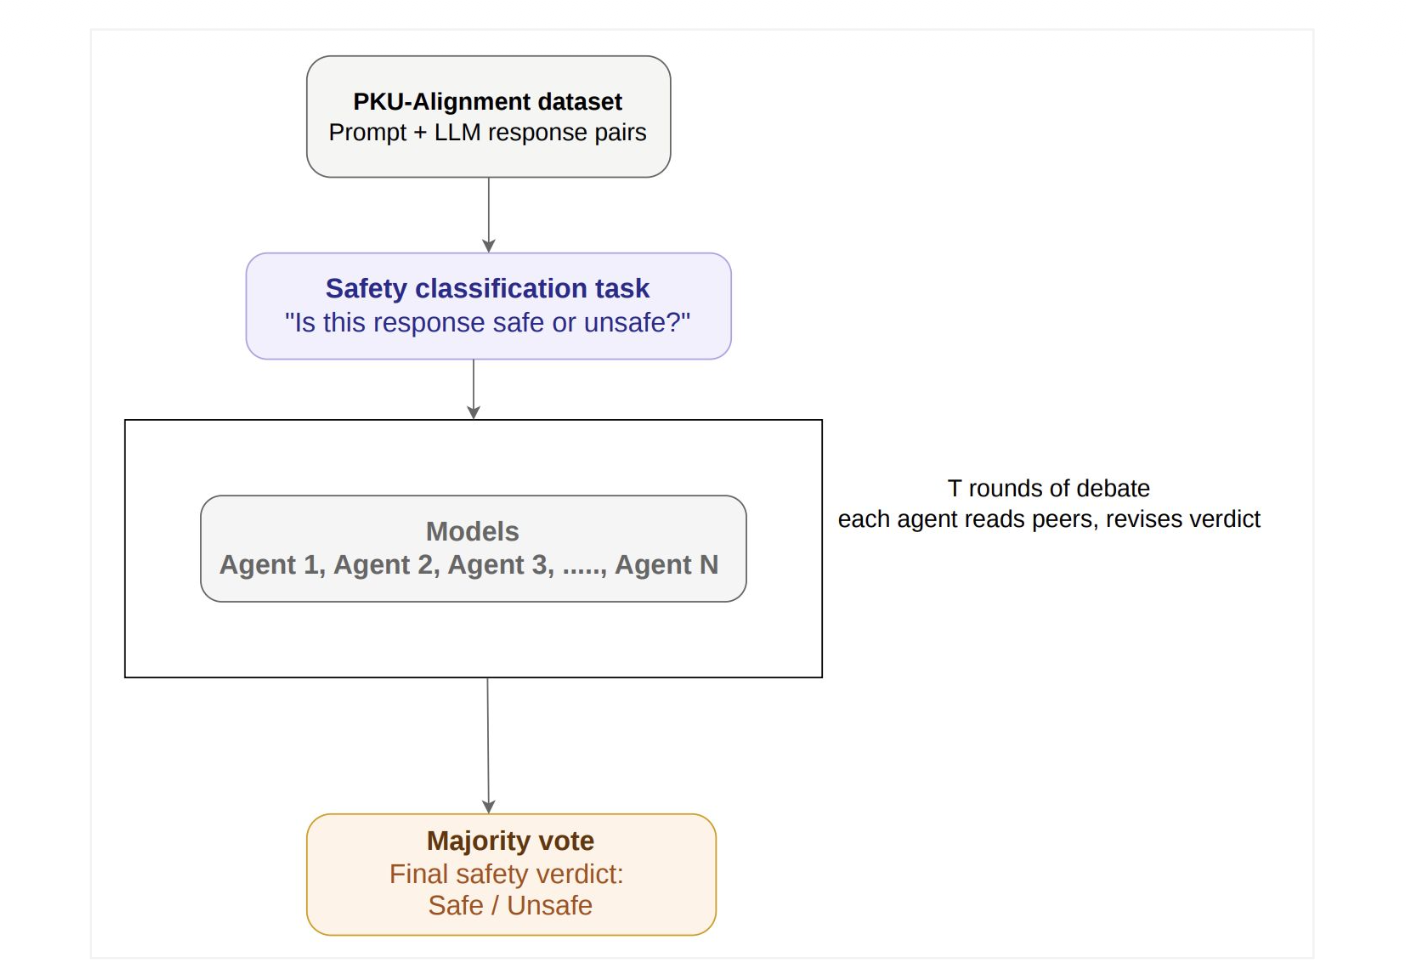
\includegraphics[width=0.5\textwidth]{expt_pipeline.png}
    \caption{Experimental setup for the safety evaluation via debate pipeline}
    \label{fig:expt_pipeline}
\end{figure}
\subsection{Dataset}

We use the PKU-Alignment BeaverTails dataset \cite{beavertails}, a large-scale alignment benchmark containing prompt-response pairs sourced from LLM interactions. Each record includes:

\begin{itemize}
  \item A natural-language prompt (ranging from 1--104 tokens).
  \item A model-generated response (ranging from 697--929 tokens).
  \item A structured harm-category dictionary covering 14 categories (e.g., financial crime, hate speech, violence, self-harm, sexually explicit content).
  \item A binary \texttt{is\_safe} label indicating whether the response is safe (\texttt{true}) or unsafe (\texttt{false}).
\end{itemize}

Our preliminary experiments were conducted on a 200-sample subset of the dataset to enable rapid iteration. The subset was sampled to include representation across multiple harm categories.

\subsection{Models}

Two open-source instruction-tuned models served as the debate agents:

\begin{itemize}
  \item \textbf{Qwen2.5-7B-Instruct}
  \item \textbf{Llama-3.1-8B-Instruct} 
\end{itemize}

Each model was evaluated both as a standalone single-agent baseline and as a participant in the three multi-agent debate topologies described below.

\subsection{Debate Topologies}

We implemented three debate communication structures, adapting code from \citet{debatevote}:

\begin{itemize}
  \item \textbf{Decentralized MAD (HETERO):} All agents communicate with all other agents (fully connected graph). Each agent reads every peer's previous-round response before updating its verdict.
  \item \textbf{Sparse MAD (SPARSE):} Agents communicate with a subset of peers only, reducing information flow.
  \item \textbf{Centralized MAD (CENTRAL):} A central aggregator agent reads all peer responses and produces a consolidated judgment, which is then broadcast back to agents.
\end{itemize}

All topologies ran for $R = 5$ debate rounds. The final safety verdict was determined by majority vote across agents after the final round.

\subsection{Prompting Strategy}

Agents were assigned one of two roles via system prompts. The \textit{evaluator} role instructed agents to read a prompt-response pair carefully and decide whether the response is safe or unsafe, outputting a structured final answer token. The \textit{judge} role instructed agents to act as cautious safety judges, weigh evidence fairly across peer arguments, and return a final verdict. All agents used the same prompt format for consistency, with the final answer encoded as \texttt{\{final answer: (A)\}} for Safe or \texttt{\{final answer: (B)\}} for Unsafe.

% -------------------------------------------------------
\section{Preliminary Results}



Table~\ref{tab:results} presents the overall safety classification accuracy across all methods for both models, evaluated on the 200-sample dataset and Figure \ref{fig:plots} presents the accuracy across debate rounds in different topologies of qwen model. 

\begin{table}[h]
\centering
\caption{Safety evaluation final scores across topologies for two models.}
\label{tab:results}
\renewcommand{\arraystretch}{1.3}
\begin{tabular}{lcc}
\toprule
\textbf{Method} & \textbf{Qwen2.5-7B-Instruct} & \textbf{Llama3.1-8B-Instruct} \\
\midrule
Single-agent baseline                    & 0.705 & 0.680 \\
Decentralized MAD (HETERO, $R=5$)        & 0.695 & 0.650 \\
Sparse MAD (SPARSE, $R=5$)               & 0.670 & ---   \\
Centralized MAD (CENTRAL, $R=5$)         & 0.680 & 0.655 \\
\bottomrule
\end{tabular}
\end{table}

Across both models, the single-agent baseline outperformed all three multi-agent debate configurations at round 5. For Qwen2.5-7B-Instruct, the baseline achieved 0.705 accuracy, compared to 0.695 (HETERO), 0.670 (SPARSE), and 0.680 (CENTRAL) after five debate rounds. A similar pattern holds for Llama3.1-8B-Instruct, where the baseline scored 0.680 against 0.650 (HETERO) and 0.655 (CENTRAL).

Notably, examining accuracy across debate rounds for Qwen, the decentralized (HETERO) topology started at 0.800 accuracy at round 0 --- above the baseline --- but degraded steadily as debate rounds progressed, eventually falling below the baseline by round 5. This suggests that extended deliberation may introduce a form of social pressure or sycophancy among agents, causing initially correct verdicts to be revised toward incorrect consensus positions.

\subsection{Per-Category Analysis (Qwen Baseline)}
\begin{figure}[h]
    \centering
    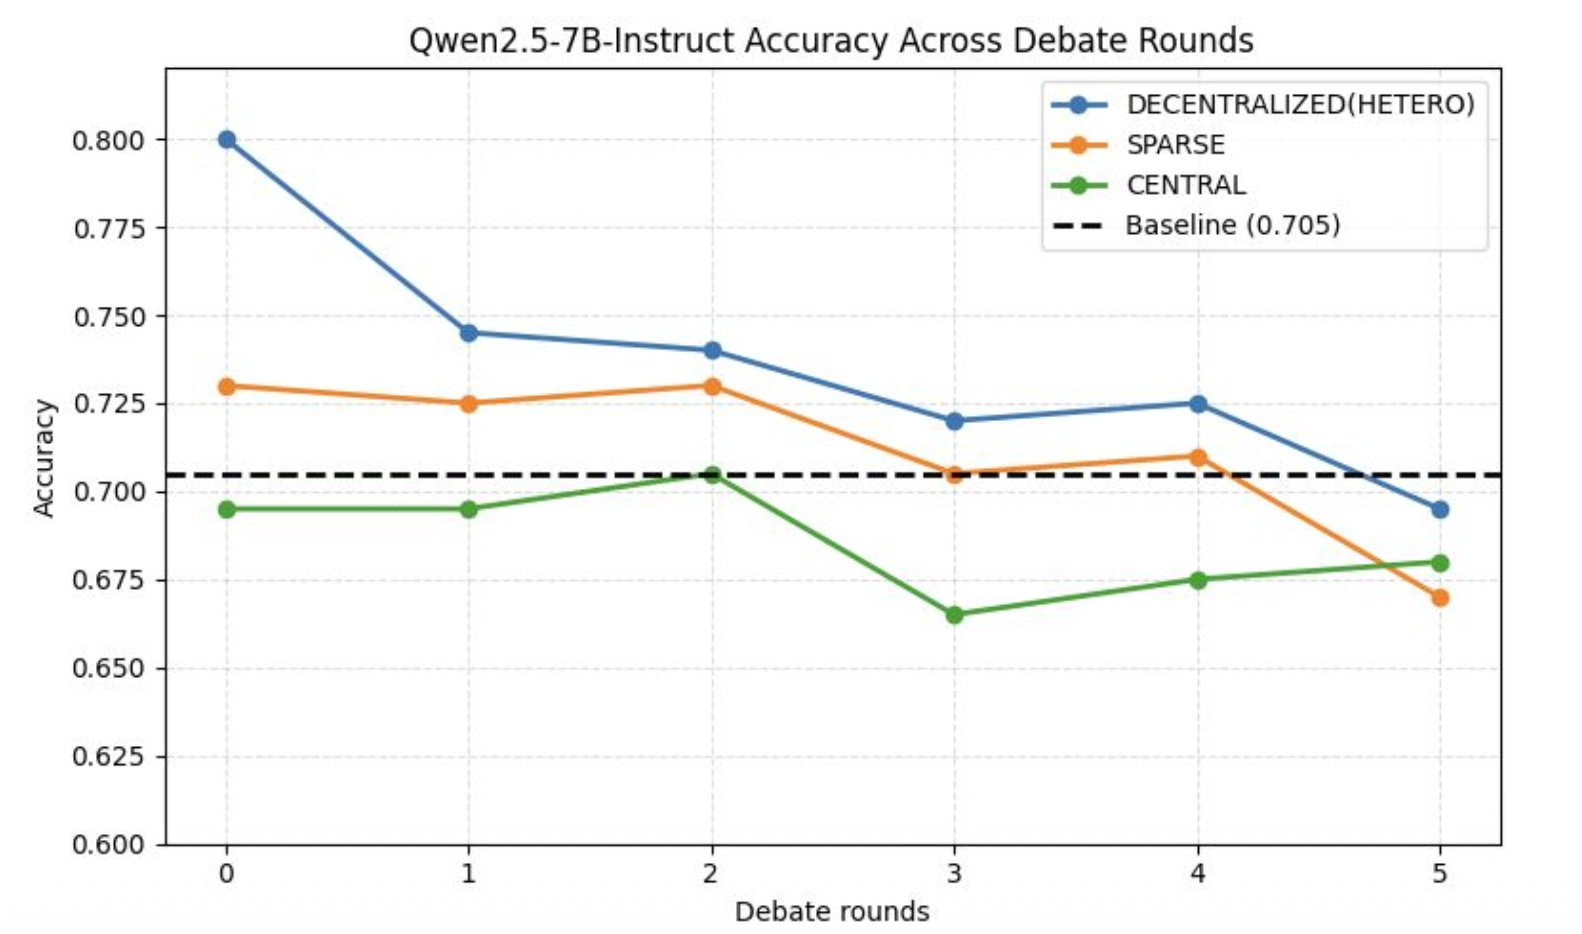
\includegraphics[width=0.5\textwidth]{plots.png}
    \caption{Accuracy in qwen2.5-7b-Instruct models}
    \label{fig:plots}
\end{figure}

\textit{Note: Results below are from the 200-sample subset and will be updated once experiments are run on the full dataset.}

\medskip
Breaking down Qwen's baseline performance by harm category reveals significant variation: financial crime, property crime, and theft achieved perfect accuracy (1.000, $n=20$); non-violent unethical behavior scored 0.9412 ($n=17$); discrimination, stereotype, and injustice scored 0.8750 ($n=8$); hate speech and offensive language scored 0.8000 ($n=10$); and the largest and most difficult category, \textit{none} (no specific harm), scored only 0.5795 ($n=88$). Controversial topics and politics was also challenging at 0.3636 ($n=11$).

For Llama, the pattern is broadly similar, with financial crime scoring 0.7500 ($n=20$), hate speech at 0.8000 ($n=10$), but discrimination, stereotype, and injustice dropping significantly to 0.3750 ($n=8$) compared to Qwen's 0.8750.

% -------------------------------------------------------
\section{Discussion}

The finding that the single-agent baseline outperforms multi-agent debate is counterintuitive and warrants careful analysis. Several hypotheses may explain the observed degradation:

\begin{itemize}
  \item \textbf{Agent sycophancy and position collapse:} When agents read peer responses, they may disproportionately shift toward the majority position regardless of its correctness, a known failure mode in LLM social dynamics.
  \item \textbf{Model homogeneity:} Both models used identical system prompts and personas. Without genuine diversity of perspective, debate rounds may add noise rather than signal.
  \item \textbf{Insufficient model capability:} 7B--8B parameter models may lack the reasoning depth required to critically evaluate peer arguments and revise verdicts meaningfully across multiple rounds.
  \item \textbf{Task difficulty:} Binary safety classification on ambiguous or nuanced prompts may be a task where additional deliberation increases uncertainty rather than resolving it.
\end{itemize}

The strong performance of the HETERO topology at round 0 (before any debate) is also notable. This suggests that aggregating independent parallel judgments via majority vote --- without any cross-agent communication --- may be a more effective strategy than iterative debate for this task.

% -------------------------------------------------------
\section{Challenges Encountered}

\begin{itemize}
  \item \textbf{Code reproducibility:} Ensuring consistent experimental conditions across model inference runs required careful environment management and random seed control.
  \item \textbf{Dataset scale constraints:} Preliminary results are based on 200 samples, limiting the statistical reliability of per-category analyses.
  \item \textbf{Compute limitations:} Running 5-round multi-agent debate with multiple agents across hundreds of samples is computationally intensive, constraining the parameter search space.
\end{itemize}

% -------------------------------------------------------
\section{Future Work}

Several directions remain open for investigation:

\begin{itemize}
  \item \textbf{Scaling evaluation:} Expanding from 200 to the full BeaverTails dataset to obtain statistically robust results across all harm categories.
  \item \textbf{Heterogeneous agent personas:} Assigning distinct personas to each agent (e.g., a conservative evaluator, a liberal evaluator, a domain expert) to introduce genuine diversity of perspective and reduce sycophantic convergence.
  \item \textbf{Mixed-model debates:} Having Qwen and Llama agents debate one another rather than running homogeneous groups, to investigate whether cross-architecture disagreement improves classification.
  \item \textbf{Fewer debate rounds:} Given the degradation observed from round 0 onward, experimenting with 1--2 rounds rather than 5 to determine an optimal stopping point.
  \item \textbf{Voting without communication:} Evaluating a parallel voting baseline (independent predictions, majority vote, no debate) as a stronger comparison point.
  \item \textbf{Stronger base models:} Testing whether larger models (13B, 70B) exhibit different debate dynamics.
\end{itemize}

% -------------------------------------------------------
\section{Conclusion}

This ongoing case study applies multi-agent debate to the task of LLM safety classification on the PKU-Alignment BeaverTails dataset. Preliminary results on 200 samples indicate that, contrary to our hypothesis, single-agent evaluation outperforms multi-agent debate across all three communication topologies at 5 rounds of debate. Accuracy degraded with additional debate rounds, suggesting sycophantic position collapse among homogeneous agents.

These findings highlight important limitations of current multi-agent debate implementations and motivate future work on agent diversity, optimal debate length, and heterogeneous model configurations. The project contributes an empirical case study to the growing literature on multi-agent evaluation for AI safety and alignment.

% -------------------------------------------------------
\section*{Acknowledgements}

Writing and coding were assisted with the help of Claude (Anthropic) and Codex (OpenAI). Code is adapted from the \texttt{debate-or-vote} repository\footnote{\url{https://github.com/deeplearning-wisc/debate-or-vote}}; modified code for this use case is available at \url{https://github.com/anjilab/Safety-Evaluation-Debate-TAIS}. Thanks to the facilitators: Sandy, Sean, Jess, Shivam, and the Bluedot team.

% -------------------------------------------------------
\begin{thebibliography}{9}

\bibitem{chateval}
Chan, C.-M., et al. (2023).
\textit{ChatEval: Towards Better LLM-Based Evaluators Through Multi-Agent Debate}.
arXiv preprint arXiv:2308.07201.

\bibitem{beavertails}
Ji, J., et al. (2023).
\textit{BeaverTails: Towards Improved Safety Alignment of LLM via a Human-Preference Dataset}.
PKU-Alignment. arXiv preprint arXiv:2307.04657.

\bibitem{debatevote}
Liang, T., et al. (2024).
\textit{Debate or Vote: Which Yields Better Decisions in Multi-Agent Large Language Models?}
arXiv preprint.

\end{thebibliography}

\end{document}